\chapter{Adversarial Anomaly Detection}\label{chap:aad}
In recent years, the use of Generative Adversarial Networks (GANs) has been explored in the context of anomaly detection. The main idea is to train a GAN to learn the distribution of the normal data and then use one or all modules to detect anomalies. This chapter presents the main concepts of GANs and how they can be used for anomaly detection in solar wind profiles. Additionally, every experiment that was undertaken with this purpose will be explained. The chapter is organized as follow:

\section{Generative Adversarial Networks}\label{sec:gan_background}
GANs were first introduced by \cite{goodfellow.etal_GenerativeAdversarialNets_} in their paper "Generative Adversarial Nets". Since then, many variations of GANs have surfaced and been applied to different areas like human face generation, image-to-image and text-to-image translation, and semantic generation, among others. The original GAN consisted of two models, a generator $G$ and a discriminator $D$. The task of the first model was to capture the distribution of the data and generate new examples from that distribution. The function of the discriminator $D$ is to distinguish actual samples from the fake data generated by $G$. The two components play an adversarial game in which $G$ tries to fool $D$ with increasingly realistic examples, and in turn, $G$ tries to detect the fake samples from $G$. The authors proposed an analogy that would help the problem's dynamics:

\noindent\textit{The generative model can be thought of as analogous to a team of counterfeiters trying to produce fake currency and use it without detection, while the discriminative model is analogous to the police trying to detect the counterfeit currency. Competition in this game drives both teams to improve their methods until the counterfeits are indistinguishable from the genuine articles.} (\cite{goodfellow.etal_GenerativeAdversarialNets_})

The problem is formulated as follows:
\begin{equation}
    \underset{G}{min}\ \underset{D}{max}\ V(D,G) = \mathbb{E}_{x \sim p_{data}(x)}[\log D(x)] + \mathbb{E}_{z \sim p_z(z)}[\log(1 - D(G(z))]
    \label{eq:gan_min_max}
 \end{equation}

 \noindent where $x$ represents the data, $z$ the latent space,  $p_{data}(x)$ is the distribution of the data and $p_z(z)$ is the distribution of the latent points (usually Gaussian) that $G$ uses to generate new samples. GANs can then be defined as a minimax game where $D$ tries to maximize $V$, as it tries to recognize generated and real images better; and, on the other hand, $G$ wants to minimize the function $V$ because its goal is to fool $G$ as many times as possible. 


\subsection{Common Challenges in the Training Phase}
Earlier GAN architectures were very unstable and hard to train. Despite some proposed solutions to these issues (\cite{radford.etal_UnsupervisedRepresentationLearning_2016,arjovsky.etal_WassersteinGenerativeAdversarial_}), GANs are still remarkably difficult to train. Following are some of the main problems experienced during this phase.\\

\noindent\textbf{Mode collapse.} Occurs when the GAN is incapable of reaching Nash equilibrium \footnote{Can be explained by the following analogy: Two players, Alice and Bob, chose strategies A and B; Alice has no other strategy to maximize her goal better, and Bob has no different strategy other than B to maximize his goal in response to Alice's choice (\url{https://en.wikipedia.org/wiki/Nash_equilibrium})} and is a consequence of poor generalization. It can occur when the generator $G$ only creates samples from a subset of the data distribution or only learns part of the distribution. The leading causes for this issue can be attributed to a poor choice of the objective function (\cite{saxena.cao_GenerativeAdversarialNetworks_2022}). In other words, $G$ focuses on a small subset of samples that consistently fool the discriminator $D$.\\

\noindent\textbf{Vanishing gradients.} The discriminator $D$ does not provide enough information for $G$ to update its gradients \cite{little.etal_GenerativeAdversarialNetworks_2021}. $D$ can distinguish real samples from fake ones with high confidence, which in turn causes the loss function of $G$ to decrease towards 0. As $D$ gets better, the gradient of $G$ progressively decreases until virtually none of the layers are updated, and $G$ can't generate samples with new distributions. Some solutions for this problem include batch normalization and clipping.\\

\noindent\textbf{Evaluation metrics.} Due to their wide range of applications, no global evaluation function can be applied to every GAN. The evaluation function varies greatly from the context of the problem in which the GAN was used. In some instances, like image generation, the principal evaluation criteria are still done qualitatively (the outputs are analyzed by humans, who determine their quality). Evaluation functions are an essential part of machine learning and allow for the correct conclusions to be made \cite{saxena.cao_GenerativeAdversarialNetworks_2022}.

%\subsection{Established GAN architectures}\label{sec:other_gans}
% TODO Wasserstein, Conditional, Bidirectional

\subsection{Anomaly Detection with GANs}\label{sec:gan_anomaly_detection}

Several approaches can be employed when using GANs for anomaly detection. The most simple one is to train both $G$ and $D$ on the normal data distribution and then use the latter to classify new samples as normal or anomalous. This is not always possible as the discriminator only learns to distinguish between samples that come from the generator and real ones. There is no guarantee that the discriminator will be able to distinguish between normal and anomalous samples, as it might have only learned specific characteristics of $G$ that are not present in the anomalous samples.

To circumvent this issue, some studies \cite{ngo.etal_FenceGANBetter_2019, liu.etal_GenerativeAdversarialActive_2020} proposed changing the focus of the vanilla GAN to be more appropriate for anomaly detection tasks. Instead of learning the normal distribution $G$ is forced to only generate anomalous samples. By forcing $G$ to generate samples close, but not equal to the normal distribution, the discriminator $D$ will learn to distinguish between normal and anomalous samples. To accommodate this, small changes to the loss functions of $D$ and $G$ are made. The results are promising, but by altering the loss functions, the new implementations might have new issues that were not experienced in other implementations.

Other studies \cite{li.etal_MADGANMultivariateAnomaly_2019, zenati.etal_AdversariallyLearnedAnomaly_2018, bashar.nayak_TAnoGANTimeSeries_2020} have proposed employing $G$ as a way to detect anomalies. These approaches are usually based on the reconstruction error of $G$ to detect anomalies, which is calculated by measuring the distance of the current sample to its closest reconstruction created by $G$. Then, an anomaly detection score can be construed with this error, either alone or in combination with the classification of the discriminator. Defective samples will, in theory, have higher reconstruction errors and will be classified as anomalous by the discriminator, as both modules didn't learn to generate or classify them correctly.

More recently, the use of adversarial autoencoders (AAE) has been proposed \cite{zenati.etal_AdversariallyLearnedAnomaly_2018,wang.etal_AdVAESelfadversarialVariational_2020} to simultaneously encode/decode an input sample and constrain its latent space representation to a prior distribution. The encoder and decoder are trained simultaneously with the discriminator, which is trained to distinguish between the latent space distribution and the prior distribution. The encoder is then used to encode new samples to the learned latent space. The discriminator classifies the latent representation of the sample as being real or fake. Similar to all other approaches, the anomaly score can be calculated by using only the reconstruction error of the decoded sample, or by combining it with the classification of the discriminator.

These methods will be employed in the experiments of this thesis. The next section explains the different approaches used to detect anomalies in solar wind profiles with the help of adversarial learning.

\section{Experiments}\label{sec:gan_experiments}
This section explains the experiments performed to detect anomalies in solar wind profiles. In total, five different architectures were used for this task. One linear GAN, three RNN-based GANs (two of which are failed experiments), and one adversarial autoencoder.

% \subsection{Anomaly Scores}\label{sec:gan_anomaly_scores}
Three anomaly detection methods are used in each experiment to detect anomalies in solar wind profiles. At the end of each experiment, the most suitable anomaly detection method was chosen based on a qualitative analysis of the results. Each approach results generates a different normality score for a given sample. The scores are then used to determine a threshold of normality based on the percentage of anomalies in the dataset. This is a hyperparameter that must be determined by the user.

The first, and simplest score is the classification of the discriminator, $D$. The values of the classification can range from 0 to 1, where values equal to 1 indicate a real sample and values closer to 0 indicate a fake label. The classification score is calculated by feeding the sample to the discriminator and obtaining the classification value. The abnormality classification score of a sample, $x$, is calculated as follows:

\begin{equation}
    D_{s} = 1 - D(x)
\end{equation}

The second score is the reconstruction error of the generator, $G$, and is based on the reconstruction technique of MAD-GAN \cite{li.etal_MADGANMultivariateAnomaly_2019}. The reconstruction process occurs iteratively for each ith sample, $x^i$ in the testing dataset. Like in the original method, the optimal latent representation for $x^i$ is obtained by first sampling a latent space variable, $z^k$. Then, for a predefined set of iterations, $j$, the generator $G$ is used to generate a batch of reconstructions $G(z^{k,j})$. Contrary to \cite{li.etal_MADGANMultivariateAnomaly_2019}, the distance between the original sample $x^i$ and the reconstructed 
one, $G(z^{k,j})$ is calculated using the MSE loss function. In the next step, the residuals of the MSE functions are averaged and used to update the parameters of $z^{k,j}$. After $j$ iterations the best reconstruction, $z^{k,j}$, of $x^i$ is returned.

The reconstruction error is calculated directly with the MSE loss between the real batch and the reconstructed batch from the optimal latent representation, $z^{k,j}$. The reconstruction error is calculated as follows:

\begin{equation}
    R_{err} = MSE(x^i, G(z^{k,j}))
\end{equation}

The reconstruction process described above is in Algorithm \ref{alg:mse_reconstruction}.
\\

\noindent\makebox[\textwidth][c]{%
\begin{minipage}{0.7\linewidth}
    \begin{algorithm}[H]
        \caption{MSE Reconstruction}\label{alg:mse_reconstruction}
    \begin{algorithmic}
        \Input
            \Desc{$x^i$}{Input Batch}
            \Desc{$n$}{Number of iterations}
        \EndInput
        \Output
            \Desc{$z^k$}{Optimal latent representation}
            \Desc{$R_{err}$}{MSE Reconstruction error}
        \EndOutput
    \end{algorithmic}

    \BlankLine
    \emph{Get a sample from the latent space}\;
    $z^k = random\_sample()$\;
    \For{$j = 0$ \KwTo $n$}{
        \emph{Reconstruct batch from $z^k$ and calculate loss}\;
        $R_{err} = MSE(x^i, G(z^k))$\;
        \emph{Update latent representation based on $R_{err}$}\;
        $z^k = update(z^k, R_{err}$)\;
        }
    \end{algorithm}
\end{minipage}}

The next score is a combination of the previous two scores, as a way of taking advantage of both the discriminator and the generator in the detection process. The reconstruction process is similar to the previous one, but instead of using only the MSE loss, the classification score, $D_{s}$ of the discriminator is also used. The new altered loss function is defined as follows:

\begin{equation}
    RD_{err} = MSE(x^i, G(z^{k,j})) \times D_{s}
\end{equation}

The reconstruction process with the discriminator input is shown in Algorithm \ref{alg:mse_reconstruction}. It is very similar to Algo. \ref{alg:mse_reconstruction}, but with the addition of the discriminator classification score to the loss function.
\\

\noindent\makebox[\textwidth][c]{%
\begin{minipage}{0.7\linewidth}
    \begin{algorithm}[H]
        \caption{MSE-Discriminator Reconstruction}\label{alg:mse_discr_reconstruction}
        \begin{algorithmic}
            \Input
                \Desc{$x^i$}{Input Batch}
                \Desc{$n$}{Number of iterations}
            \EndInput
            \Output
                \Desc{$z^k$}{Optimal latent representation}
                \Desc{$RD_{err}$}{MSE-Discr. Reconstruction error}
            \EndOutput
        \end{algorithmic}
        
        \BlankLine
        \emph{Get a sample from the latent space}\;
        $z^k = random\_sample()$\;
        \For{$j = 0$ \KwTo $n$}{
            \emph{Obtain $D$ classification for reconstructed batch}\;
            $D_s = 1 - D(G(z^k))$\;

            \emph{Reconstruct batch from $Z^k$ and calculate loss}\;
            $RD_{err} = MSE(x^i, G(z^k)) \times D_s$\;
            \emph{Update latent representation based on $RD_{err}$}\;
            $z^k = update(z^k, RD_{err}$)\;
        }
    \end{algorithm}
\end{minipage}}


A simplified representation of the workflow for obtaining the anomaly scores is shown in Figure \ref{fig:anomaly_detection_method}. This process is done by extracting the pre-trained $G$ and $D$ with their layers frozen. Each batch, $x^i$ is passed through the discriminator, $D$, to obtain the classification score, $D_s$. The reconstruction process from algorithms \ref{alg:mse_discr_reconstruction} and \ref{alg:mse_reconstruction} is performed in the invert mapping step to obtain the optimal latent representation, $z^k$, for the given test sample. After this, $R_{err}$ is calculated by comparing the reconstructed sample with the original one. The final $RD_{err}$ can be obtained by combining $R_{err}$ with $D_s$.


\begin{figure}[]
    \centering
    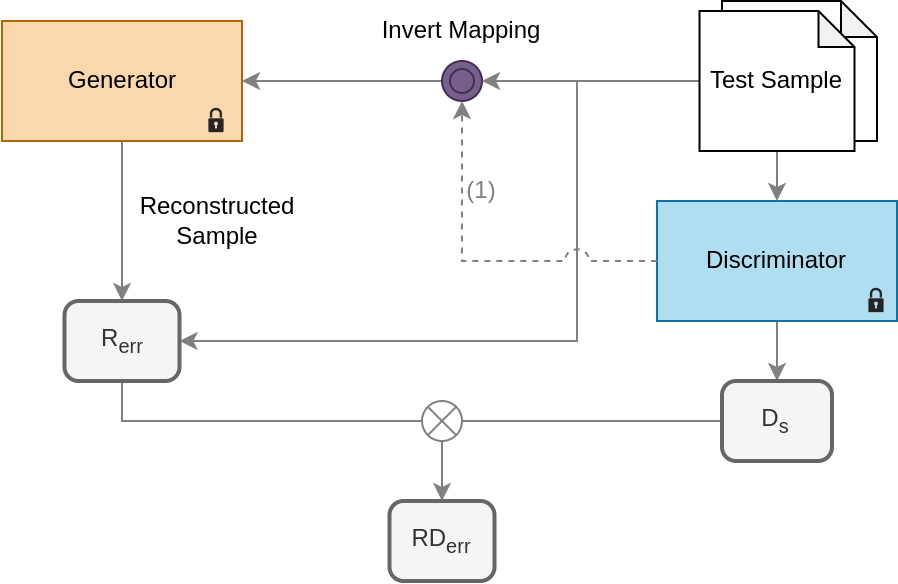
\includegraphics[width=0.8\textwidth]{figures/gan_anomaly_detect_flow.png}
    \caption[Anomaly detection workflow]{Anomaly detection workflow with each of the defined reconstruction methods. The invert mapping is used to obtain the optimal latent representation, $z^k$, from the reconstruction error.}\label{fig:anomaly_detection_method}
    \small\textsuperscript{(1)} Only applied to the reconstruction method in algorithm \ref{alg:mse_discr_reconstruction}.
\end{figure}



\subsection{Linear GAN}\label{sec:linear_gan}

\begin{figure}
    \centering
    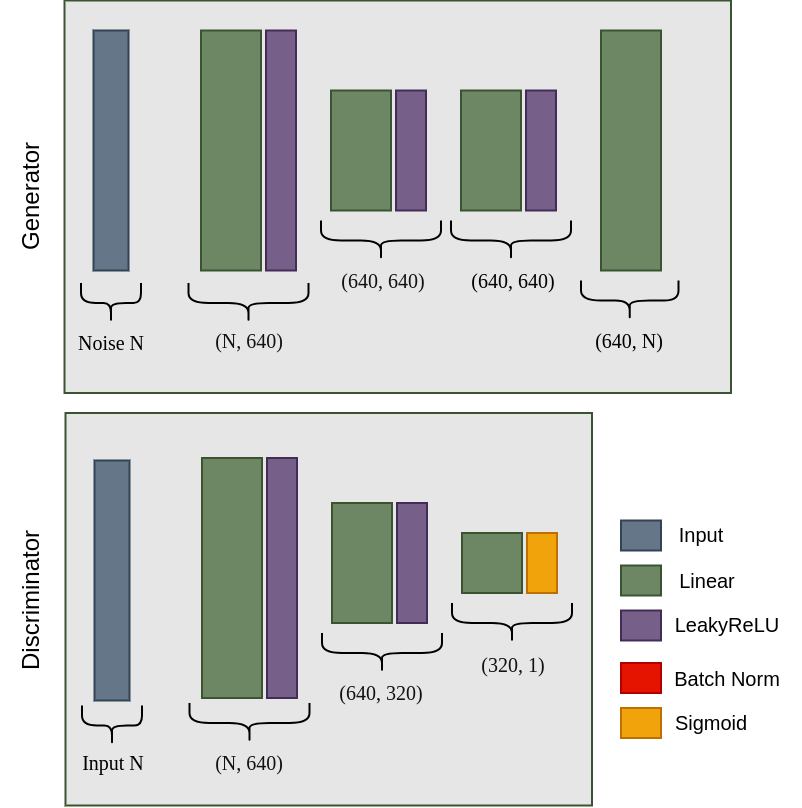
\includegraphics[width=0.8\textwidth]{figures/linearGAN.png}
    \caption{Linear GAN Architecture}
    \label{fig:linear_gan_architecture}
\end{figure}


The first architecture was a linear GAN, which is a simple GAN with a linear generator and discriminator. Several experiments were performed with different configurations of the architecture. The use of BatchNorm in either module was tested, to try and stabilize the training process. This proved to be ineffective as it made it difficult for $G$ and $D$ to converge. Because of this, it was not included in the final implementation. In addition to this, the number of intermediate stacked linear layers was varied during the tests to try and find a configuration that worked best for this problem. 

Besides these changes, different activation functions were also tested. The activation functions used were ReLU, LeakyReLU, and Tanh, with a combination of them in the intermediate as well as in the output and input layers. Similar to other GAN architectures, the LeakyReLU activation function was chosen to prevent the gradient from vanishing, and to improve the overall stability of the learning process. Most configurations that included the Tanh activation function in the output layer of the generator were discarded, as it proved to not be effective during the anomaly detection phase.

The final architecture is shown in Fig. \ref{fig:linear_gan_architecture}. Both the generator and discriminator are built with linear layers. The generator, $G$, consists of an input layer that takes as input a latent space variable, $Z$ with $L_P$ features, and outputs a sample with the same dimension as the input. The first layer performs a linear transformation on the input noise vector and projects $Z$ into lower dimensional space with 640 dimensions. The output of this layer is then passed through a LeakyReLU activation function. Next, the resulting features from this step are passed through two stacked linear layers, each with 640 dimensions. In the last layer, the features from the previous step undergo a linear transformation to project them into the same dimension as the input sample. As was previously said, no activation function is used in the output layer of the generator, as it was not effective during the detection phase.

The discriminator, $D$, consists of an input layer that takes as input a sample with $L_P$ features and outputs a scalar value. The objective of $D$ is to progressively learn the most important features of the data to perform binary classification of the input sample as being real or fake. The first and subsequent layers perform linear transformations of the input data into increasingly smaller dimensions. In the output layer, the features from the previous step are projected into a single scalar value. This value is then passed through a sigmoid activation function to obtain the final classification score of each sample.

\subsubsection*{Training}
Both modules were trained with the Adam optimizer with a learning rate of 0.0001 for the generator and 0.0002 for the discriminator. This was done to prevent the discriminator from overpowering the generator during the training process. The weights of each of the linear layers were initialized with the He initialization function from \cite{He.Zhang.ea_DelvingDeepRectifiers_2015}.

Two models were trained, the first one, $M_i$, to detect anomalies in the inputs of the MULTI-VP dataset and the other, $M_o$, for the outputs (refer to Chapter \ref{chap:eda}). Both models were trained over 300 epochs with a batch size of 128. In both approaches the training data was scaled with the \textit{MinMaxScaler} to preserve the variation of extreme values in the data. The training data consisted of a matrix with $N\times L_P$ dimension, where $N$ is the number of training samples and $L_P$ is the number of features per profile. Like in the clustering experiments, the selected validation data was excluded from the training process, for further use. 

From Section \ref{chap:eda} we know that every variable in a profile has 640 features, so the total number of features per sample can be defined as $L_P = k\times 640$, where $k$ is the number of variables in a profile that is used during training. 

In $M_i$, the input data, $X_i$, consists of the concatenation of the $B [G]$ and $\alpha [deg]$ variables of each profile. The radial coordinate radius, $R [R_{sun}]$ was excluded from the process, to reduce the number of features the networks needed to learn. In addition to this, extreme variations in the input data were removed to prevent both modules from learning noisy features that would hinder the detection process. Following the previous notation, the number of features for each sample is $L_{P_i} = 2\times 640 = 1280$.

In the outputs model, $M_o$, every output variable of MULTI-VP is used in the training phase. Each sample consists of the concatenation of the density, $n [10^{10}cm^{-3}]$,  the velocity, $v [km/s]$, and temperature, $T [MK]$, with a combined number of features per sample, $L_{P_o}$, of 1920. Contrary to the input model, no extreme variations were removed from the data, as it performed well without this step.

\subsubsection*{Anomaly Detection}
The detection step was carried out for each of the models with all three anomaly score functions defined in the beginning of this section. Due to the lack of validation metrics, the choice of method was based on the visual inspection of the results. The stability of the anomaly scores as well as the quality of the dataset without anomalies were taken into account.

With these criteria in mind, the best results were obtained with the reconstruction error, $R_{err}$. The other two functions, $D_{s}$ and $RD_{err}$, were very unstable and were not able to detect the anomalies as well as $R_{err}$. The filtered input and output variables can be seen in Image \ref{fig:linear_gan_clean_in} and \ref{fig:linear_gan_clean_out} respectively.


\begin{figure}[]
    \caption[Linear GAN filtered datasets]{Resulting datasets after the anomaly detection step with the linear GAN architecture on the inputs and outputs of the MULTI-VP dataset.}
    \label{fig:linear_gan_clean_data}
    \begin{subfigure}[h]{0.6\textwidth}
        \centering
        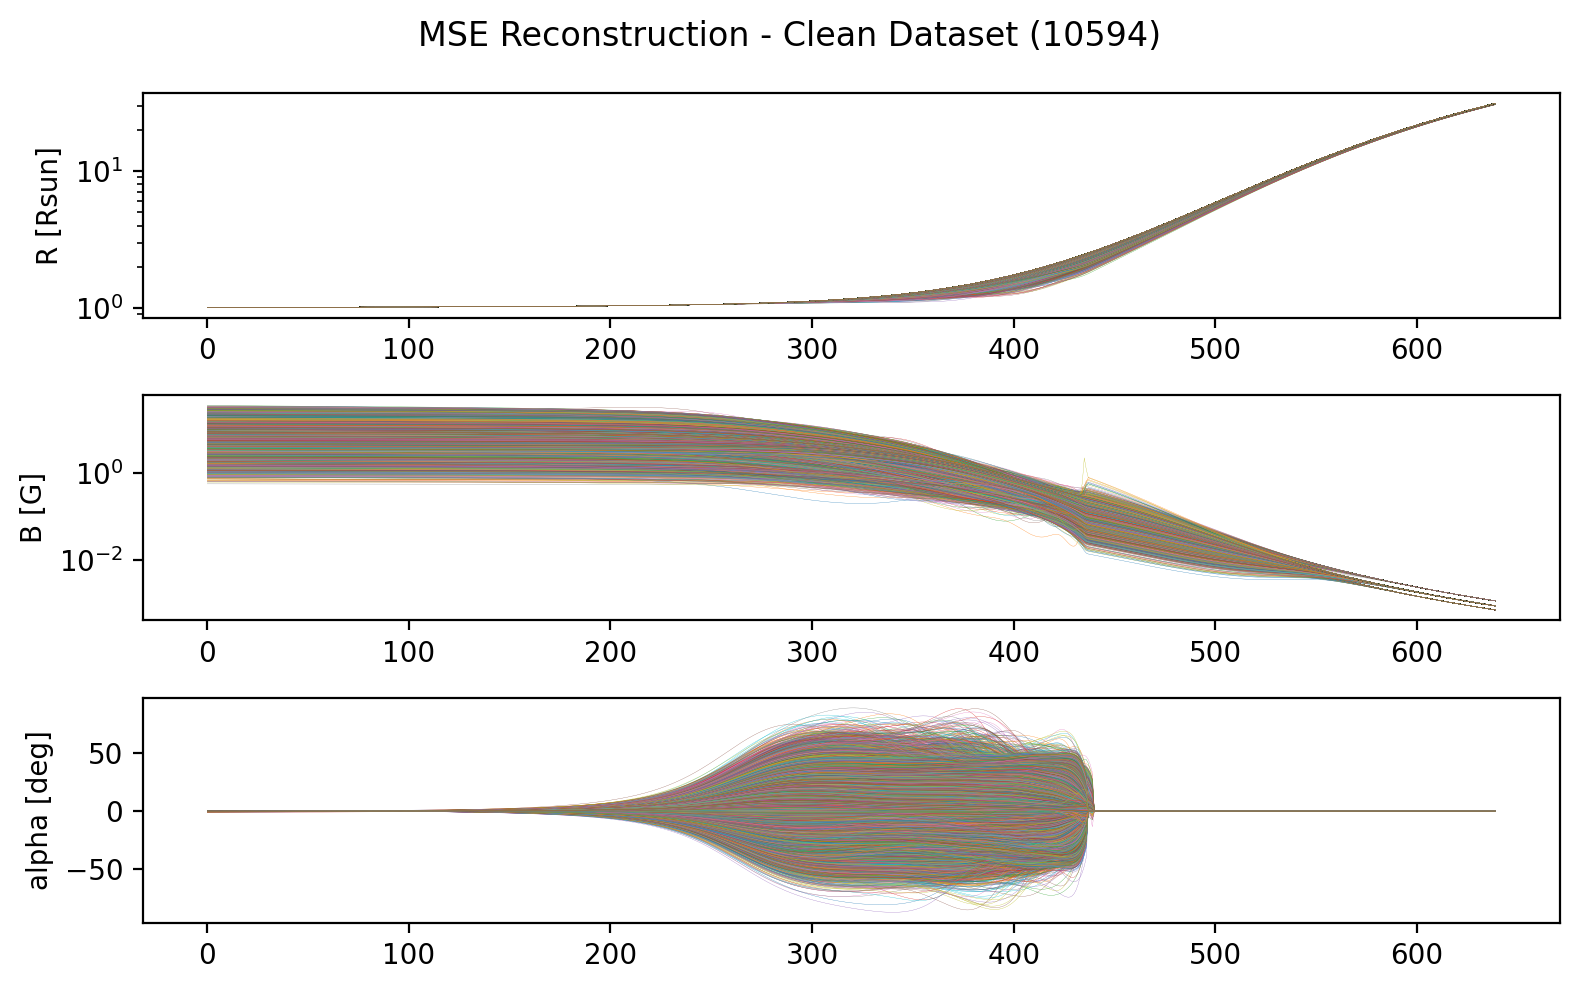
\includegraphics[width=\textwidth]{figures/linearGAN_clean_in.png}
        \caption{Input Variables}
        \label{fig:linear_gan_clean_in}
        % \label{fig:tsne_mag_2d}
    \end{subfigure}
    \hfill
    \begin{subfigure}[h]{0.6\textwidth}
        \centering
        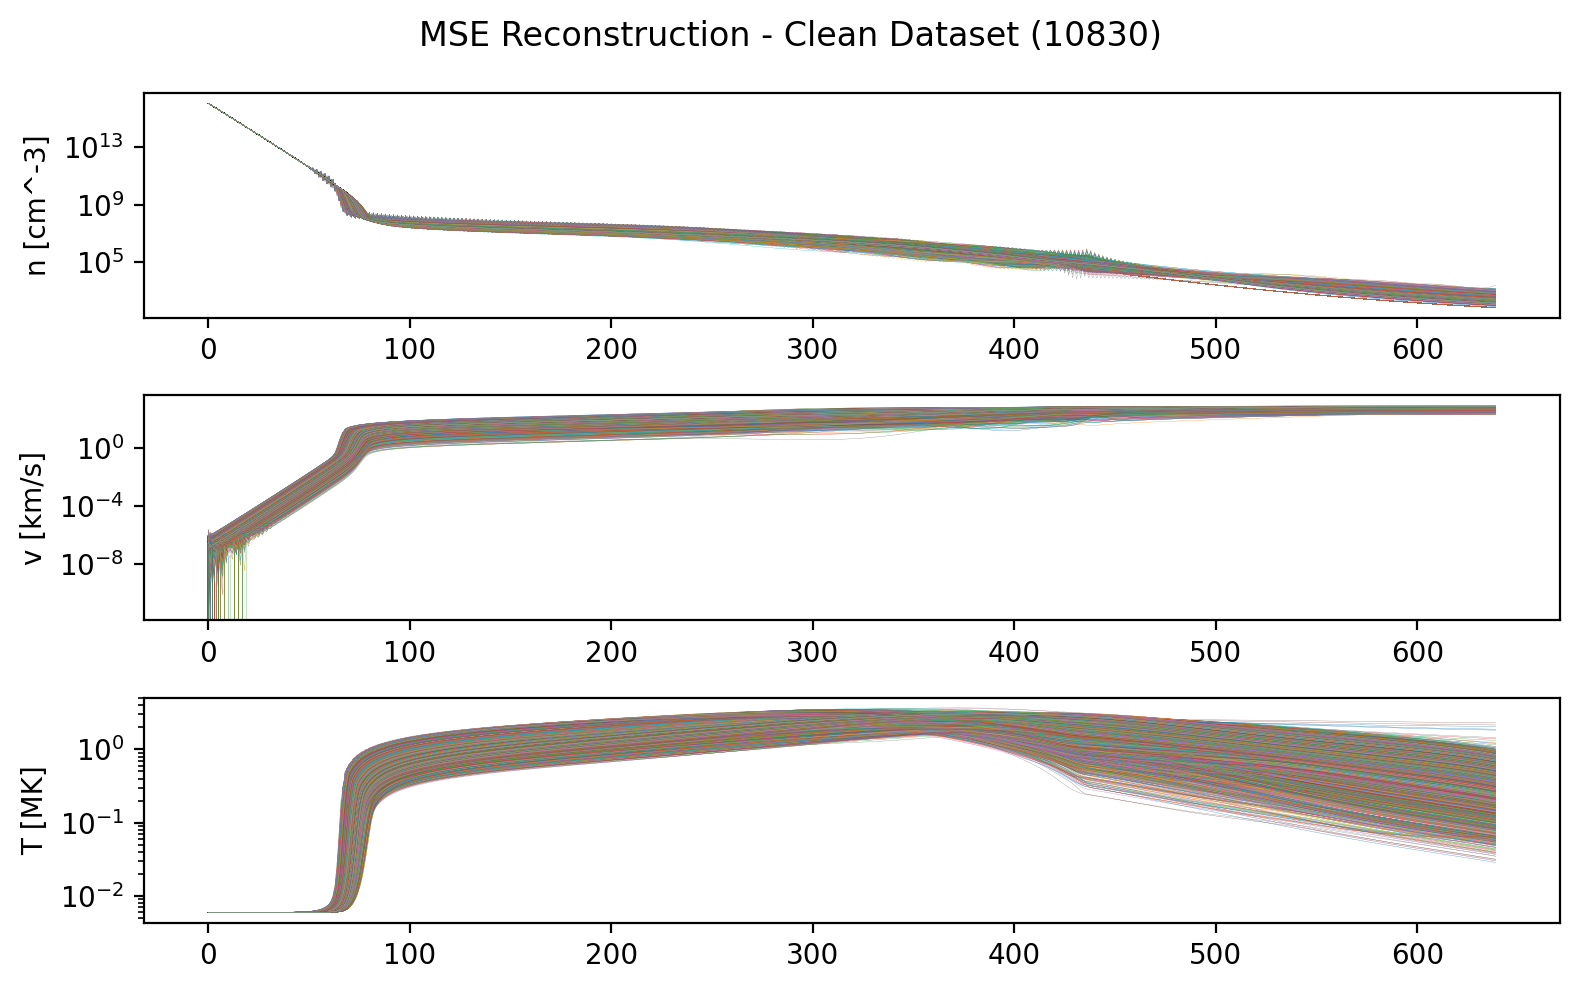
\includegraphics[width=\textwidth]{figures/linearGAN_clean_out.png}
        \caption{Output Variables}
        \label{fig:linear_gan_clean_out}
    \end{subfigure}
\end{figure}

The first image (Fig. \ref{fig:linear_gan_clean_in}) resulted from removing 10\% of the files from the original dataset based on anomaly scores. As was previously said, the anomaly scores were obtained by training the GAN model, $M_i$ in the input variables and then using $G$ to calculate the anomaly scores of each sample in the testing dataset. The results show that the data is mostly clean, with some anomalies remaining in the magnetic field, $B [G]$, variable.

For the output variables (Fig. \ref{fig:linear_gan_clean_out}) only 8\% of the files were excluded based on anomaly scores. The resulting output variables are mostly clean, with some abnormalities in the density, $n [cm^3]$, variable.

Overall, the experiments with this architecture prove that it can detect anomalies in the input and output variables of MULTI-VP. However, the percentage of files that need to be removed (i.e. the False Positive rate) is still very high. This might indicate that the current architecture might not be the most ideal for the task, as seemingly "normal" profiles might be excluded from the prediction step.


\subsection{Failed RNN-based GANs}\label{sec:gan_experiment_lstm}
The next experiments were with RNN-based GANs. These experiments are based on the assumption that consecutive profiles in the MULTI-VP dataset are somewhat similar but have small variances. This can be closely associated with other studies for the detection of anomalies in time-series data (refer to Section \ref{sec:sota_anomaly_detection}). 

Several architectures were designed and tested first with the RNN-based GANs. These failed to produce any meaningful results as the GANs were very unstable during training and the anomaly scores were not able to detect any anomalies in the data. This might be due to the issues associated with traditional RNN-based architectures, such as the vanishing gradient problem \cite{Schmidt_RecurrentNeuralNetworks_2019}.

Having this into consideration, the next batch of tests was carried out with GRU-based GANs. GRU NNs, like LSTM NNs, can learn long-term dependencies in the data sequences. However, they are less resource intensive and faster to train than LSTM NNs as they require fewer parameters. The results obtained with the GRU architectures were tested with LSTM ones, to ensure that the results were not biased by the choice of architecture. The performance of both architectures was similar, with the GRU-based GANs being slightly faster to train. Because of this, the results presented in this section are from GRU GAN architectures, as they are more efficient than LSTM ones, and reach similar outcomes.

\subsubsection*{Stacked GRU GAN}
Before reaching a stable RNN architecture, several experiments were carried out with different architectures. The first attempts consisted of employing multilayer GRUs for both $G$ and $D$. Several iterations were tried with a different number of recurrent layers and hidden sizes. Due to the high number of features, $L_P$, of the input data, several tests were carried out with deep multilayer GRUs. However, the results were not satisfactory as the GANs were very unstable during training. $D$ would always outperform $G$ in this phase, causing the latter to collapse and produce meaningless results. This occurred even when $D$ had significantly fewer layers than $G$. In addition, reducing the learning rate of the discriminator didn't seem to affect the instability of the GANs. 

Having these issues into consideration, other configurations of the network were tested by reducing the number of features that were given to the stacked GRU layers. This was done by applying a linear transformation on the input data that significantly reduced the dimensionality of the data. With this layer, in theory, only the most important attributes of the inputs would be retained and passed to the subsequent layers. This approach managed to improve the stability of the GANs during training, but the results of the detection phase were still subpar with the ones from the linear GAN.

\subsubsection*{Pyramid GRU GAN}
In the second batch of experiments, and as a way of circumventing the dimensionality issues of the stacked GRU GAN, a pyramid GRU GAN was designed. This architecture consisted of a simple generator with three GRU layers and an output linear layer for activation.
The first wot layers would narrow the input size to smaller dimensions, to make sure that only the most meaningful features would be retained. Then the last GRU layer would upscale the outputs from the previous layers into a higher dimension. In the output layer, the resulting features would suffer from a linear transformation that transformed the data into the desired output dimension of the generator. This would then be passed through the Tanh activation function.
    
The first attempts consisted of using a simple Generator with four GRU layers. The first two layers would narrow the input size to smaller dimensions and then, the last layer would upscale the features into a higher dimension. Then, in the output layer, the features from the previous GRU layers would be passed through a Linear layer that would transform the data into the desired output dimension of the generator. The transformed data was then passed through the Tanh activation function. 

The discriminator consisted of only two GRU and a linear output layer. Following the same logic as the generator, the first two layers, progressively reduced the number of features of the input data. The output layer would reduce the features from the last layer to just one, which would then be passed through the sigmoid activation function for binary classification.

As in the previous experiments, the training process of the GAN became more stable; however, the results of the anomaly detection still weren't as good as the ones obtained by the linear GAN.





% \subsection{Stacked GRU GAN}
% The first attempts consisted of employing multilayer GRUs for both $G$ and $D$. Several attempts were tried with a different number of recurrent layers and hidden sizes. Due to the high number of features, $M$ of the input data, several tests were carried out with deep multilayer GRUs. However, the results were not satisfactory as the GANs were very unstable during training. $D$ would always outperform $G$ in this phase, causing the latter to collapse and produce meaningless results. This occurred even when $D$ had significantly fewer layers than $G$. In addition, reducing the learning rate of the discriminator didn't seem to affect the instability of the GANs. 

% Having these issues into consideration, other configurations of the network were tested by reducing the number of features that were given to the stacked GRU layers. This was done by applying a linear transformation on the input data that significantly reduced the dimensionality of the data. With this layer, in theory, only the most important attributes of the inputs would be retained and passed to the subsequent layers. This approach managed to improve the stability of the GANs during training, but the results of the detection phase were still subpar with the ones from the linear GAN.

% \subsection{Pyramid GRU GAN}\label{sec:pyramid_gru_gan}

% As a way of circumventing the dimensionality issues of the stacked GRU GAN, a pyramid GRU GAN was designed. This architecture consisted of a simple generator with three GRU layers and an output linear layer for activation.
% The first wot layers would narrow the input size to smaller dimensions, to make sure that only the most meaningful features would be retained. Then the last GRU layer would upscale the outputs from the previous layers into a higher dimension. In the output layer, the resulting features would suffer from a linear transformation that transformed the data into the desired output dimension of the generator. This would then be passed through the Tanh activation function.

% The first attempts consisted of using a simple Generator with four GRU layers. The first two layers would narrow the input size to smaller dimensions and then, the last layer would upscale the features into a higher dimension. Then, in the output layer, the features from the previous GRU layers would be passed through a Linear layer that would transform the data into the desired output dimension of the generator. The transformed data was then passed through the Tanh activation function. 

% The discriminator consisted of only two GRU and a linear output layer. Following the same logic as the generator, the first two layers, progressively reduced the number of features of the input data. The output layer would reduce the features from the last layer to just one, which would then be passed through the sigmoid activation function for binary classification.

% As in the previous experiments, the training process of the GAN became more stable; however, the results of the anomaly detection still weren't as good as the ones obtained by the linear GAN.


\subsection{MAD-GAN}\label{sec:madgan}

\begin{figure}
    \centering
    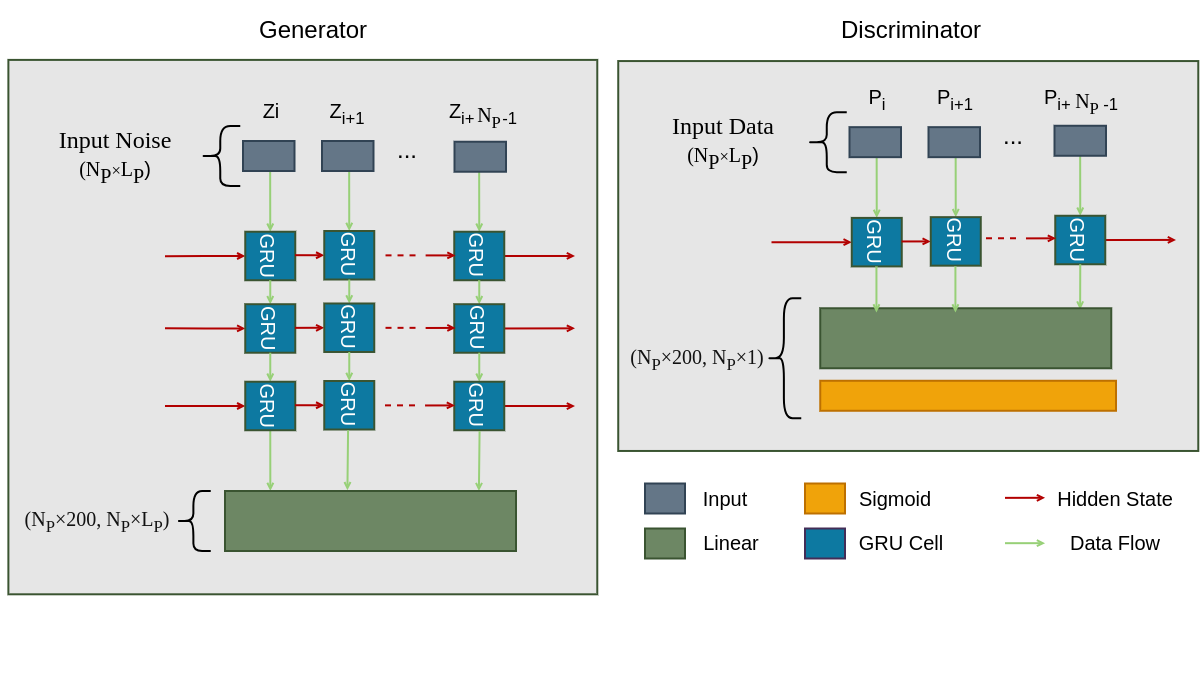
\includegraphics[width=0.8\textwidth]{figures/madgan_arch.png}
    \caption[MAD-GAN Architecture]{Architecture of the MAD-GAN model. The Generator consists of three stacked GRU layers and a linear output layer. The discriminator consists of a single GRU layer and a linear output layer followed by the Sigmoid activation function. Both take as input sequences of size $N_P$.}
    \label{fig:madgan_architecture}
\end{figure}

The definitive architecture for this class of GANs was based on MAD-GAN \cite{li.etal_MADGANMultivariateAnomaly_2019}. It was chosen as a way of determining if one of the most famous state-of-the-art RNN GANs for time-series data could be used for the detection of anomalies in the MULTI-VP dataset. The architecture of the generator and discriminator is shown in Figure \ref{fig:madgan_architecture}.

Like in \cite{li.etal_MADGANMultivariateAnomaly_2019} the generator, $G$, consists of three stacked GRU layers and a linear output layer (without an activation function). The discriminator, $D$, consists of a single GRU layer and a linear output layer followed by the Sigmoid activation function. $G$ takes as inputs windows with $N_P$ latent vectors with $L_P$ features and synthesizes samples with the same dimensions. $D$ takes as inputs windows with $N_P$ real or fake samples with $L_P$ features and outputs a single value between 0 and 1, which represents the probability of the input window coming from the dataset or $G$.

\subsubsection*{Data Preparation}
Unlike the previous architecture, the data is aggregated into windows, $W$, with consecutive profiles. The size of each window, $N_P$, is a hyperparameter that needs to be tuned. and indicates the number of consecutive profiles, $P$, that are fed into the GANs. With this formulation, the ith window, $W_i$, is defined as the set of the $N_P$ consecutive profiles of the ith profile, $P_i$, in the dataset, such that $W_i = \{P_i, P_{i+1}, ..., P_{i+N_P-1}\}$.

Each window varies in length, $L_P$, according to the number of variables that are used for anomaly detection. Each variable in the dataset has an equal number of features (refer to Section \ref{sec:data_prelim_analysis}); therefore, the number of features for a single profile can be expressed as $L_P=k\times 640$, where $k$ is the number of variables being used for the task. From this, the dimensions of the ith window, $W_i$, can be defined as $(N_P, L_P)$.

As in the previous experiments, two models were designed to detect anomalies in both the input and output variables used by MULTI-VP. In the model trained on the inputs ($M_i$) only the magnetic field, $B [G]$ variable was used for the task at hand. This was due to the problems faced in the previous RNN experiments (sec. \ref{sec:gan_experiment_lstm}) due to the high dimensionality of the dataset. Additionally, the magnetic field is the variable in the dataset that seems to be most affected by the presence of anomalies. Following the notation adopted in the last paragraph, the dimensions of the ith window, $W_{i}$, in the dataset is set to $(N_P, 640)$, where 640 is the number of features $L_P$ of the $B [G]$ variable and $N_P$ is the window size.

In line with the previous experiments, the most extreme values from the input variables were removed from the training process to ensure the best performance of the GAN models. These were then used during the detection phase.

Additionally, the output model, $M_o$ was trained on the three output variables of the MULTI-VP dataset without removing extreme values. With this, the dimension of each window in the training dataset is set to $(N_P, 1920)$, where 1920 is the number of features $L_P$ of the three output variables and $N_P$ is the window size.

\subsubsection*{Training}
Several configurations were tested for the number of hidden units for the GRU layers. The best results were obtained with 200 hidden units in both modules. The learning rate was set to 0.0001 for $G$ and 0.0002 for $D$ with the use of the Adam Optimizer. The batch size was set to 32 and the number of epochs to 100. The number of profiles per window, $N_P$, was set to 10. In addition to this, the same training method as in \cite{li.etal_MADGANMultivariateAnomaly_2019} was used. In this method, $D$ is firstly trained for a set number of iterations while $G$ is kept fixed. This is to ensure that $D$ learns the representation of the real data before training $G$. After this, $G$ is trained for a set number of iterations while $D$ is kept frozen. This process is repeated until the end of the training process. The number of iterations was 10 and 5 for $D$ and $G$, respectively.

As in the previous RNN architectures, the training process was very unstable and the modules didn't converge due to the high number of input features. Changing the number of hidden features, the learning rate and the number of iterations didn't seem to affect the stability of the training process.

In an attempt to reduce the number of features of data and in line with the additional experiments in \cite{li.etal_MADGANMultivariateAnomaly_2019}, PCA was applied to the training data. This transformation reduced the number of features, $L_P$, to a fixed 100 features per profile. For the model $M_i$, the initial 640 features from the magnetic field variable were reduced to 100 features. For $M_o$, the 1920 features from all the output variables were reduced to 100 features. With this, the dimension of both training windows was set to ($N_P, 100$).

\subsubsection*{Anomaly Detection}
The detection step for both models was carried out with the three anomaly functions defined earlier. Every anomaly score function provided overall good results, showcasing the stability of the method. Despite this, the best results were obtained with the $R_{err}$ function. The results of the anomaly detection on the inputs as well as on the outputs are shown in Figure \ref{fig:madgan_clean_data}. These were obtained by first training the models with the PCA-transformed data and then applying the anomaly detection step on the testing data with the model from the previous stage.

\begin{figure}
    \caption[MAD-GAN filtered datasets]{Resulting datasets after the anomaly detection step with the MAD-GAN architecture on the inputs and outputs of the MULTI-VP dataset.}
    \label{fig:madgan_clean_data}
    \begin{subfigure}[h]{0.6\textwidth}
        \centering
        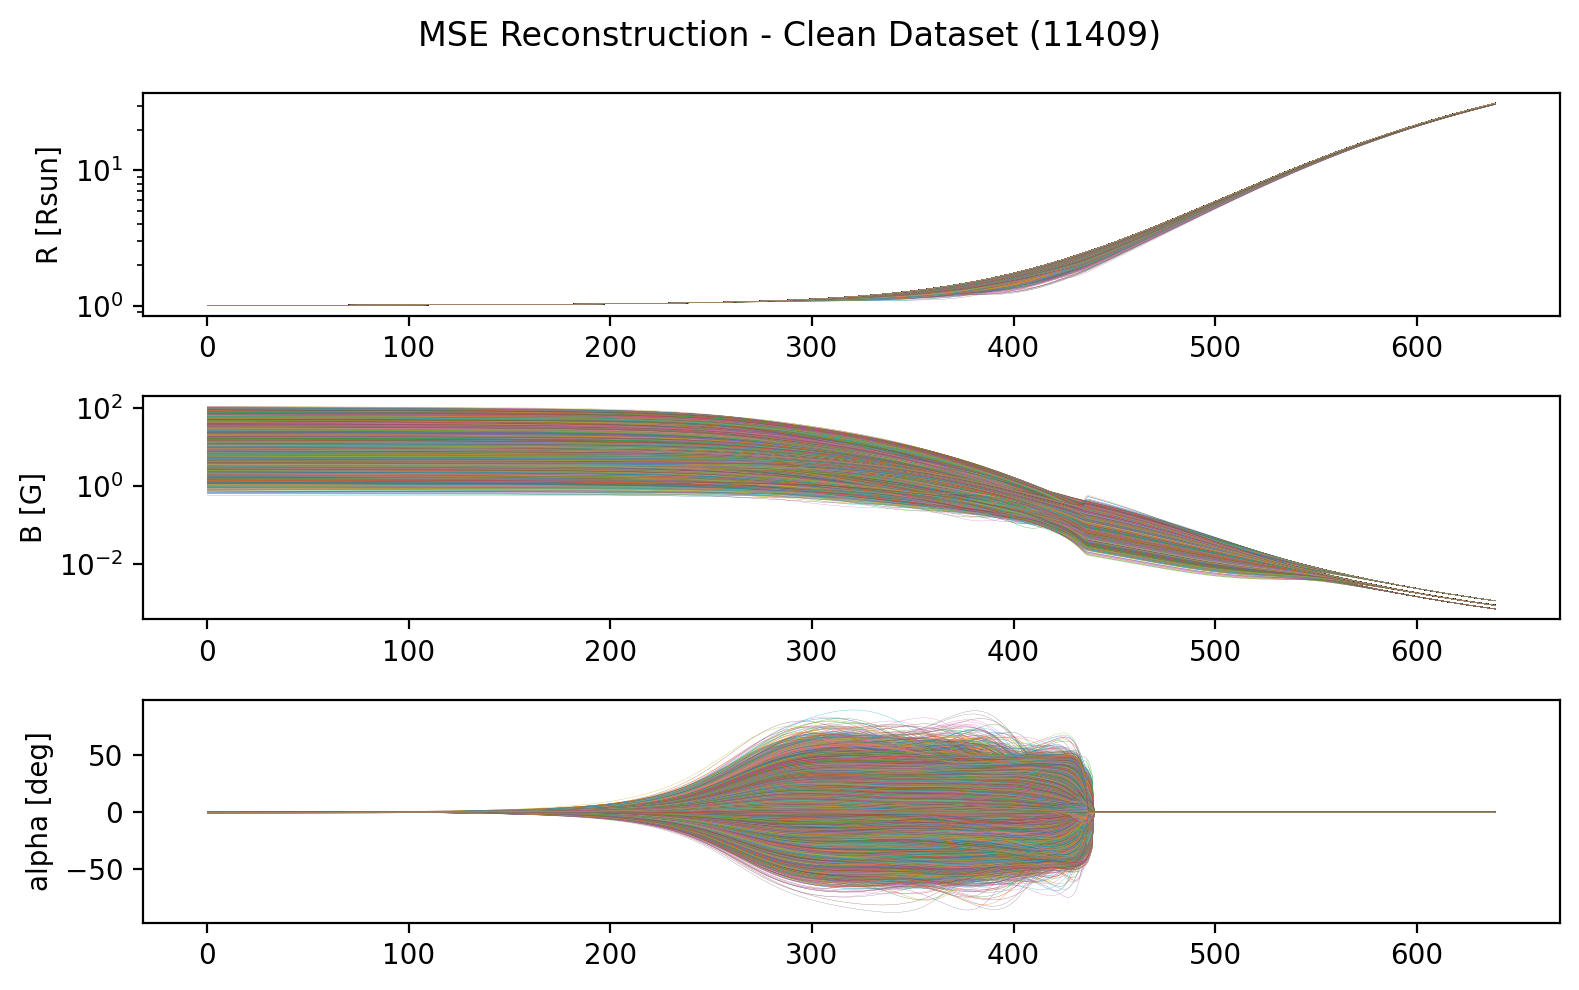
\includegraphics[width=\textwidth]{figures/madgan_clean_in.png}
        \caption{Input Variables}
        \label{fig:madgan_clean_in}
        % \label{fig:tsne_mag_2d}
    \end{subfigure}
    \hfill
    \begin{subfigure}[h]{0.6\textwidth}
        \centering
        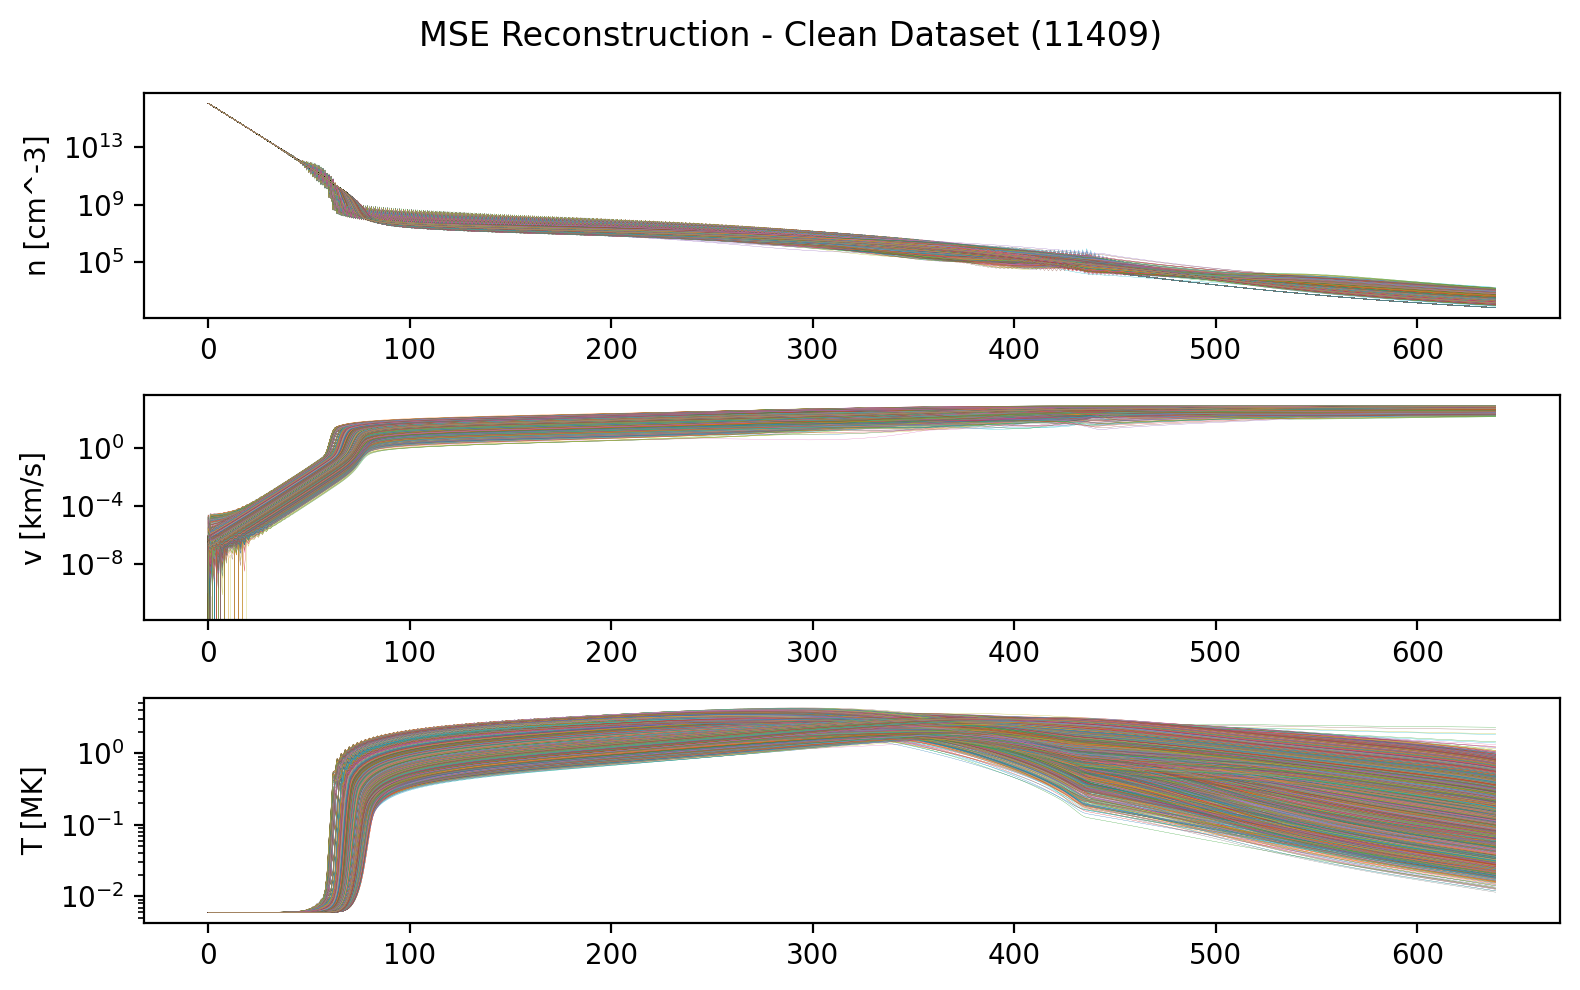
\includegraphics[width=\textwidth]{figures/madgan_clean_out.png}
        \caption{Output Variables}
        \label{fig:madgan_clean_out}
    \end{subfigure}
\end{figure}

Figure \ref{fig:madgan_clean_in} shows the results of the anomaly detection on the input variables. At first glance, the results are very similar to the ones obtained with the linear GAN; however, MAD-GAN only required a threshold of 3\% top anomalous profiles. This means that the model is more sensitive to anomalies in the magnetic field variable than the linear GAN model. The same is true for the model trained on the output variables (fig. \ref{fig:madgan_clean_out}). These results indicate that MAD-GAN is more sensitive to anomalies in both the input and output variables than the linear GAN model, which translates to a lower False-Positive rate.

Note that these results were only possible because of the use of PCA. This might indicate that the experiments in Section \ref{sec:gan_experiment_lstm} might have worked if the same method was employed. A possible issue with this approach is that PCA might be removing important features from the data, which could be used to improve the results of the anomaly detection step.

\subsection{Adversarial AE}\label{sec:aae}
In the final experiments, an adversarial autoencoder architecture was used. This architecture was chosen as a way of determining if the use of an autoencoder could improve the results obtained with the previous GAN architectures. The architecture of the generator and discriminator is shown in Figure \ref{fig:aae_architecture}. 

\begin{figure}
    \centering
    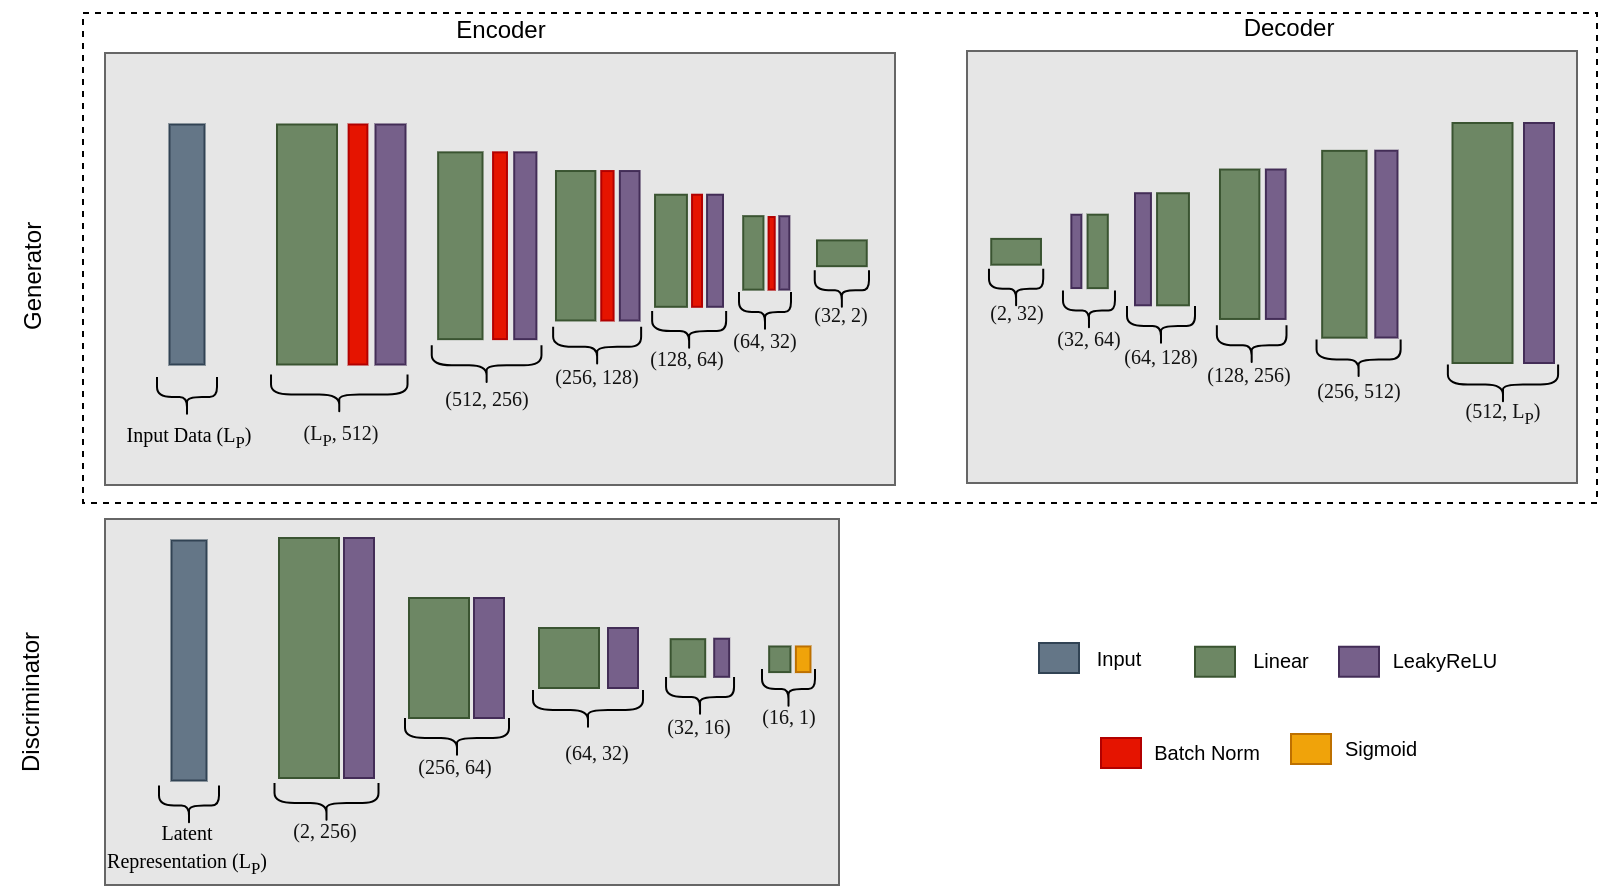
\includegraphics[width=0.8\textwidth]{figures/aae_arch.png}
    \caption[Adversarial Autoencoder Architecture]{Architecture of the adversarial autoencoder. The generator $G$, consists of an encoder, $Enc$, and decoder, $Dec$. The job of the first is to generate a latent representation of the input data, which is then used by the decoder to reconstruct the input. The discriminator, $D$, takes as inputs the latent representation generated by $Enc$ and outputs a single value between 0 and 1, which represents the probability of the input coming from the prior distribution or $Enc$.}
    \label{fig:aae_architecture}
\end{figure}

The generator, $G$, is divided into an encoder, $Enc$, and decoder $Dec$. The objective of $Enc$ is to generate a latent representation of the input data. This latent representation is then used by $Dec$ to reconstruct the input data. In adversarial autoencoders, a discriminator model is also introduced to constrain the latent representation to follow a prior distribution. In this case, the discriminator, $D$, takes as input the latent representation generated by $Enc$ and outputs a single value between 0 and 1, which represents the probability of the input coming from the prior distribution or $Enc$.

\subsubsection*{Training}

The loss function combines the reconstruction loss of the autoencoder (Equation \ref{eq:ae_objective_func}) with the adversarial loss of the discriminator. The reconstruction loss is the mean squared error between the input to de encoder and the output of the decoder. The adversarial loss is the binary cross-entropy loss between the output of the discriminator and the prior distribution. The loss function is defined as follows:

\begin{equation}\label{eq:aae_objective_func}
    \mathcal{L}_{AAE} = \alpha \times \mathcal{L}_{AE} + (1-\alpha) \times \mathcal{L}_{ADV}
\end{equation}

where $\alpha$ is a hyperparameter that controls the weight of the reconstruction and adversarial losses.

The training process consists of first training the autoencoder and freezing the discriminator parameters. In this step, the encoder, $Enc$ generates a latent space representation of the original data, which is then reconstructed by the decoder, $Dec$. The parameters of the encoder and the decoder are updated with the equation \ref{eq:aae_objective_func}. After this, $D$ is trained while the encoder and decoder are kept frozen. In this step, the discriminator is trained to distinguish between the latent representation generated by the encoder and the prior distribution. With this, $D$ is conditioned to learn the prior distribution and to classify the encoded samples more precisely. This process is repeated until the end of the training process.

In this phase, the AAE was trained over 400 epochs with the help of the Adam Optimizer, with a learning rate of 0.0002 for $D$, and 0.0001 for $G$. The batch size was set to 128 and the hyperparameter $\alpha$ was set to 0.999. The prior distribution was set to two separate 2D Gaussian distributions. 

Like in the previous experiments, a model was trained for the input variables and another for the output variables. For the first, only the magnetic field variable (without extreme values) was used as input, while for the second, all the output variables were used.

\subsubsection*{Anomaly Detection}

The anomaly detection step was carried out with the same anomaly functions as in the previous experiments; however, the generator reconstruction step is done directly with the autoencoder without the need for the construction steps of the previous approaches.


The autoencoder proved more than capable of detecting anomalies in the data without the need for a discriminator. However, as previously stated, the goal of this approach is to take advantage of the reconstruction abilities of the autoencoder along with the discriminator to improve the results of the baseline autoencoder. The results of the anomaly detection step are shown in Figure \ref{fig:aae_clean_data}.

\begin{figure}
    \caption[AAE filtered datasets]{Resulting datasets after the anomaly detection step with the AAE architecture on the inputs and outputs of the MULTI-VP dataset.}
    \label{fig:aae_clean_data}
    \begin{subfigure}[h]{0.6\textwidth}
        \centering
        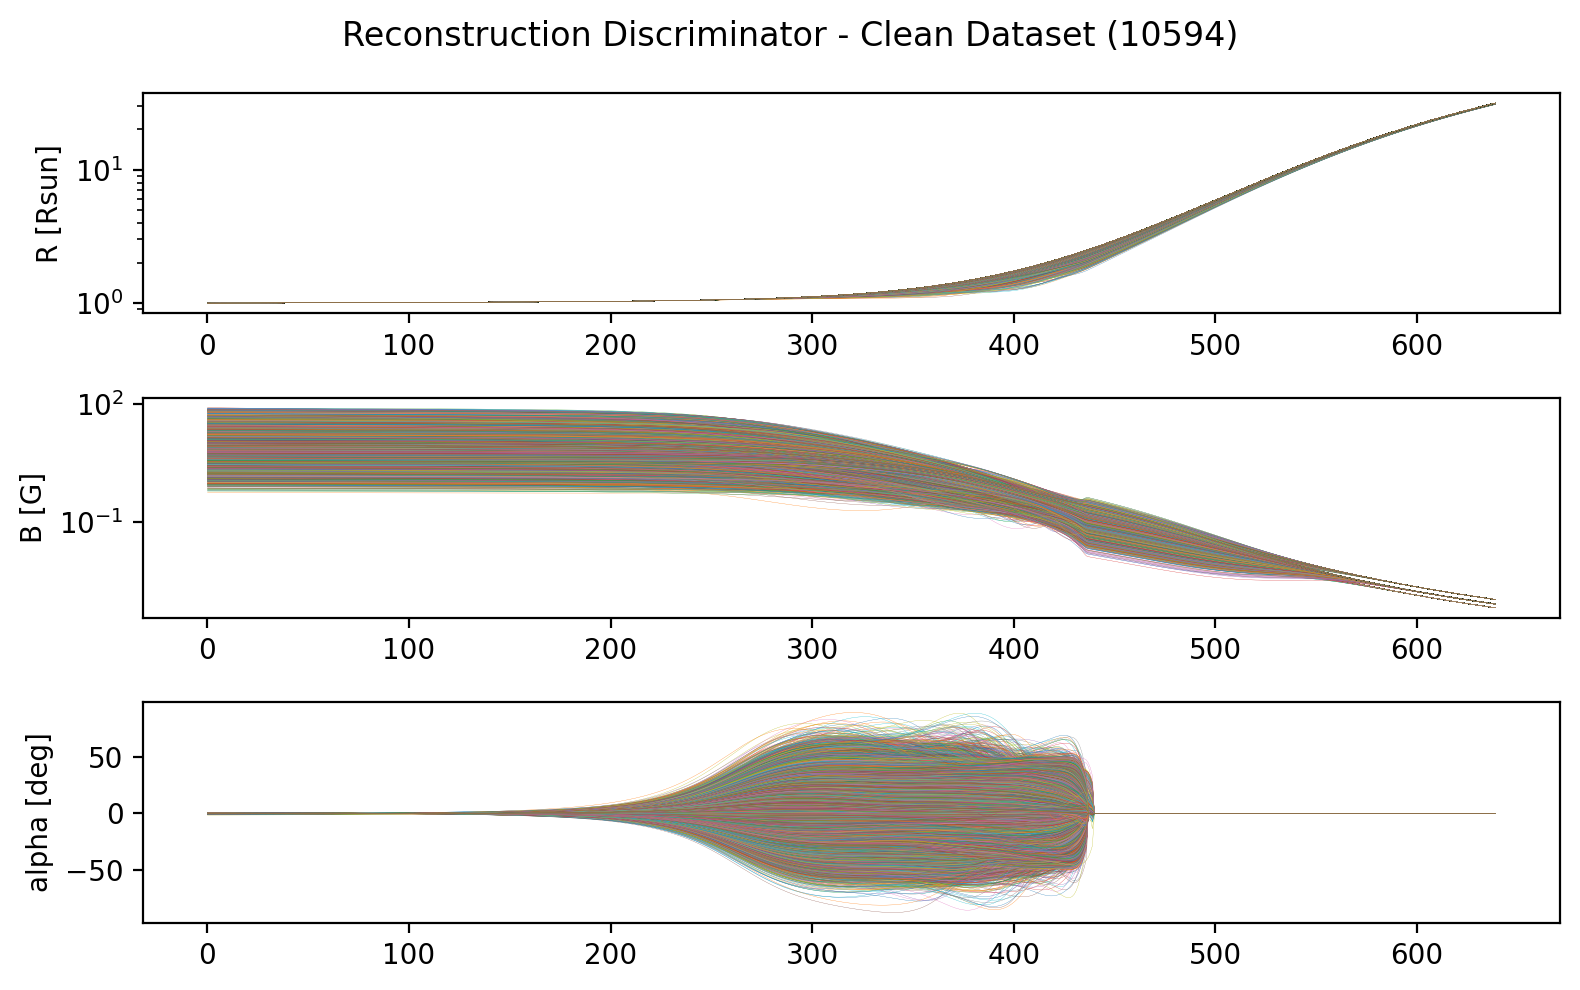
\includegraphics[width=\textwidth]{figures/aae_clean_in.png}
        \caption{Input Variables}
        \label{fig:aae_clean_in}
        % \label{fig:tsne_mag_2d}
    \end{subfigure}
    \hfill
    \begin{subfigure}[h]{0.6\textwidth}
        \centering
        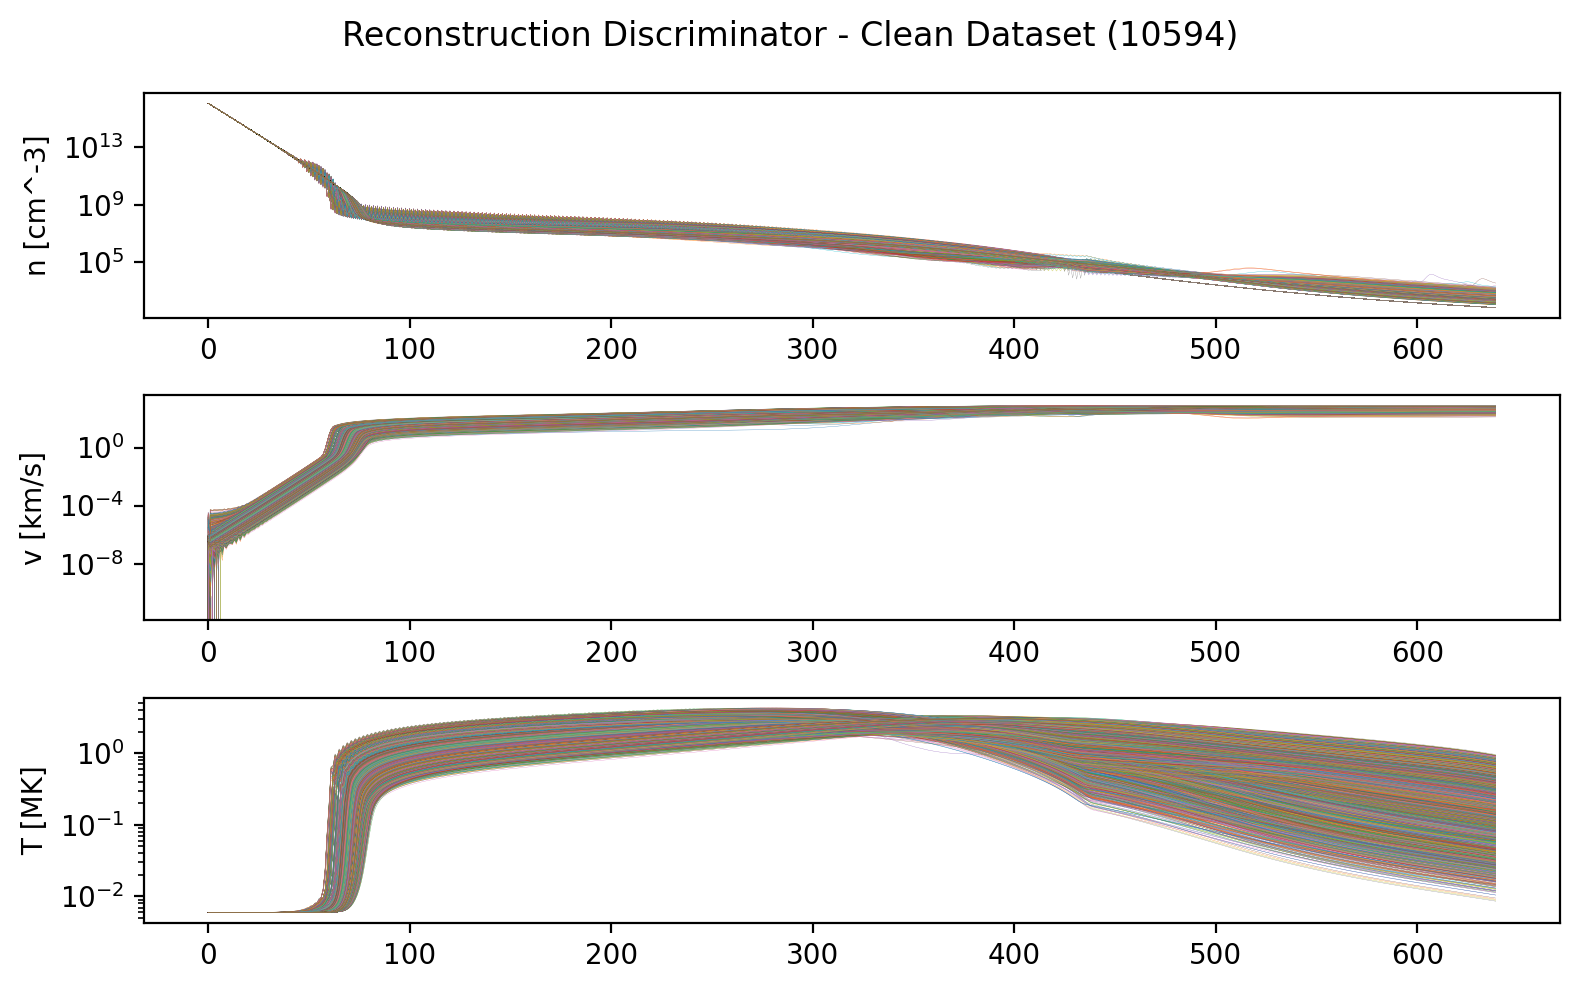
\includegraphics[width=\textwidth]{figures/aae_clean_out.png}
        \caption{Output Variables}
        \label{fig:aae_clean_out}
    \end{subfigure}
\end{figure}

The results show similar outcomes as in the linear GAN implementation. Both images were obtained by removing the top 10\% anomalous profiles from the dataset. The results show that the AAE is capable of detecting anomalies in the input and output variables. However, the results are not as good as the ones obtained with the MAD-GAN.


\subsection{Experiments Summary}\label{gan_experiments_summary}

\begin{table}[]
\caption{Summary of the results obtained with the different GAN architectures.}\label{tab:gan_results}
\begin{threeparttable}[b]
\begin{tabular}{@{}crrrlrrr@{}}
\toprule
\multicolumn{1}{l}{} & \multicolumn{3}{c}{Input Variables}                                                               &  & \multicolumn{3}{c}{Output Variables}                                                         \\ \cmidrule(lr){2-4} \cmidrule(l){6-8} 
\multicolumn{1}{l}{} & \multicolumn{1}{c}{Function} & \multicolumn{1}{c}{Threshold (\%)} & \multicolumn{1}{c}{Anomalies} &  & \multicolumn{1}{c}{Function} & \multicolumn{1}{c}{Threshold} & \multicolumn{1}{c}{Anomalies} \\ \cmidrule(lr){2-4} \cmidrule(l){6-8} 
Linear GAN           & Rerr                         & 10                                 & 1177                          &  & Rerr                         & 8                             & 941                           \\
MAD-GAN              & Rerr                         & 3                                  & 352                           &  & Rerr                         & 3                             & 352                           \\
AAE                  & RDerr\tnote{1}                        & 10                                 & 1177                          &  & RDerr\tnote{1}                        & 10                            & 1177                          \\ \bottomrule
\end{tabular}
\begin{tablenotes}
    \item [1] Direct reconstruction error from the generator ($Enc+Dec$) without algorithm \ref{alg:mse_discr_reconstruction}.
\end{tablenotes}
\end{threeparttable}
\end{table}

A summary of the results obtained in the detection phase with the different GAN architectures is shown in Table \ref{tab:gan_results}. From an analysis of the results, MAD-GAN managed to clean the dataset with the smallest anomaly threshold. The next best architecture was Linear GAN, with the same threshold in the input variables as in AAE, but with a lower threshold in the outputs. Despite these architectures having the same anomaly threshold for the input variables, some anomalies remained in the dataset that resulted from the linear GAN. This might indicate that the anomaly threshold for this approach should have been higher than 10\%.

In conclusion, MAD-GAN proved to be the best architecture in the anomaly detection step. It managed to clean the dataset with the smallest anomaly threshold, this way preserving the most normal profiles in the dataset. The resulting datasets from this step will be used in the prediction phase, described in the next section.


\section{ML Experiments}\label{ml_experiments}
In line with the results from the previous section, the prediction phase was carried out with the datasets obtained from the MAD-GAN architecture. The same procedure as in Section \ref{sec:clustering_ml_experiments} was followed. The same clustering division was used for consistency; however this time the datasets were filtered by the chosen anomaly detection method before the training step. 

